%-----------------------------------------------------------------------------
% plotfiles
%-----------------------------------------------------------------------------
\section{Plotfiles}

\maestro\ outputs plotfile specifically for visualization and analysis.
Table~\ref{vis:table:plotfile} lists the quantities stored in a plotfile.
Not all of these may be present, dependent on what options were used in 
creating the plotfile.

By default, plotfiles store double precision data, but if
\runparam{single\_prec\_plotfiles} {\tt = T} is set, then the data is
converted to single precision before outputting---this is done to
reduce file sizes.

\renewcommand{\arraystretch}{1.3}
{\footnotesize
\begin{center}
\begin{longtable}{|l|p{2.25in}|p{2.5in}|}

\caption{Plotfile quantities}
\label{vis:table:plotfile} \\
%
\hline \multicolumn{1}{|c|}{\textbf{plotfile variable name}} & 
       \multicolumn{1}{|c|}{\textbf{description}} & 
       \multicolumn{1}{|c|}{\textbf{runtime parameter controlling output}} \\ \hline
\endfirsthead

\multicolumn{3}{c}%          
{{\tablename\ \thetable{}---continued}} \\
\hline {plotfile variable name} & 
       {description} & 
       {runtime parameter controlling output} \\ \hline
\endhead

\multicolumn{3}{|r|}{{\em continued on next page}} \\ \hline
\endfoot

\hline
\endlastfoot

{\tt x\_vel}   & $\ut$  & -- \\
%\hline
{\tt y\_vel}   & $\vt$  & -- \\
%\hline
{\tt z\_vel}   & $\wt$  & 3-d runs only \\
%\hline
{\tt density}  & $\rho$ & -- \\
%\hline
{\tt rhoh}   & $(\rho h)$ & {\tt use\_tfromp = F} or ({\tt use\_tfromp = T} and \runparam{plot\_h\_with\_use\_tfromp} {\tt = T}) \\           
%\hline
{\tt h}      & $(\rho h)/\rho$   & {\tt use\_tfromp = F} or ({\tt use\_tfromp = T} and {\tt plot\_h\_with\_use\_tfromp = T}) \\           
%\hline
{\tt X(*)}   & $(\rho X_k)/\rho$ & \runparam{plot\_spec} \\
%\hline
{\tt tracer} & tracers           & \runparam{plot\_trac} \\
%\hline
{\tt w0\_x}  & $w_0 \er \cdot \ex$ & \runparam{plot\_base} \\ 
%\hline
{\tt w0\_y}  & $w_0 \er \cdot \ey$ & {\tt plot\_base} \\ 
%\hline
{\tt w0\_z}  & $w_0 \er \cdot \ez$ & {\tt plot\_base} \\ 
%\hline
{\tt divw0}  & $\nabla \cdot w_0$  & {\tt plot\_base} \\ 
%\hline
{\tt rho0}   & $\rho_0$            & {\tt plot\_base} \\ 
%\hline
{\tt rhoh0}  & $(\rho h)_0$         & {\tt plot\_base} \\ 
%\hline
{\tt h0}     & $(\rho h)_0/\rho_0$  & {\tt plot\_base} \\ 
%\hline
{\tt p0}     & $p_0$                & {\tt plot\_base} \\ 
%\hline
{\tt radial\_velocity}  & $\Ubt \cdot \er + w_0$ & \runparam{spherical} {\tt == 1} \\
%\hline
{\tt circum\_velocity}  & $| \Ubt - (\Ubt \cdot \er) \er |$ &  {\tt spherical == 1}  \\
%\hline
{\tt magvel}              & $| \Ubt + w_0 \er |$  & -- \\
%\hline
{\tt momentum}            & $\rho | \Ubt + w_0 \er |$  & -- \\
%\hline
{\tt vort}                & $| \nabla \times \Ubt |$   & -- \\
%\hline
{\tt S}                   & $S$   & -- \\
%\hline
{\tt rhopert}             & $\rho - \rho_0$  & -- \\
%\hline
{\tt rhohpert}          & $(\rho h) - (\rho h)_0$ & {\tt use\_tfromp = F} or ({\tt use\_tfromp = T} and {\tt plot\_h\_with\_use\_tfromp = T}) \\           
%\hline
{\tt tfromp}              & $T(\rho, p_0, X_k)$  & -- \\
%\hline
{\tt tfromh}            & $T(\rho, h, X_k)$    & {\tt use\_tfromp = F} or ({\tt use\_tfromp = T} and {\tt plot\_h\_with\_use\_tfromp = T}) \\           
%\hline
{\tt deltaT}            & $[T(\rho, h, X_k) - T(\rho, p_0, X_k)]/T(\rho, h, X_k)$  & {\tt use\_tfromp = F} or ({\tt use\_tfromp = T} and {\tt plot\_h\_with\_use\_tfromp = T}) \\           
%\hline
{\tt deltap}            & $|p(\rho,h,X_k) - p_0|/p_0$ & {\tt use\_tfromp = F} or ({\tt use\_tfromp = T} and {\tt plot\_h\_with\_use\_tfromp = T}) \\           
%\hline
{\tt tpert}               & $T(\rho,h,X_k) - \overline{T}$ if {\tt use\_tfromp = F}; $T(\rho,p_0,X_k) - \overline{T}$ otherwise & -- \\
%\hline
{\tt Machnumber}          & $| \Ubt + w_0 \er | / c(\rho,p_0,X_k)$ & -- \\
%\hline
{\tt soundspeed}        & $c(\rho,p_0,X_k)$ & \runparam{plot\_cs} \\
%\hline
{\tt deltagamma}          & $\Gamma_1(\rho,p_0,X_k) - \gammabar$ & -- \\
%\hline
{\tt entropy}             & $s(\rho,p_0,X_k)$ & -- \\
%\hline
{\tt entropypert}         & $[s(\rho,p_0,X_k) - \overline{s}]/\overline{s}$ & -- \\
%\hline
{\tt sponge} or {\tt sponge\_fdamp} & $1/(1 + \Delta t \kappa f_\mathrm{damp})$ by default; $f_\mathrm{damp}$ if \runparam{plot\_sponge\_fdamp = T} & -- \\
%\hline
{\tt pi}                 & $\pi$ & -- \\
%\hline
{\tt gpi\_x}           & $\nabla \pi \cdot \ex$ & \runparam{plot\_gpi} \\
%\hline 
{\tt gpi\_y}           & $\nabla \pi \cdot \ey$ & {\tt plot\_gpi} \\
%\hline
{\tt gpi\_z}           & $\nabla \pi \cdot \ez$ & {\tt plot\_gpi} \\
%\hline
{\tt pioverp0}         & $\pi / p_0$ & {\tt plot\_base} \\
%\hline
{\tt p0pluspi}         & $p_0 + \pi$ & {\tt plot\_base} \\
%\hline
{\tt omegadot(*)}      & $\dot{\omega}_k$ & \runparam{plot\_omegadot} \\
%\hline
{\tt enucdot}          & $(\rho \Hnuc)/\rho$ & \runparam{plot\_Hnuc} \\
%\hline
{\tt Hext}             & $(\rho \Hext)/\rho$ & \runparam{plot\_Hext} \\
%\hline
{\tt eta\_rho}         & $\etarho$ & \runparam{plot\_eta} \\
%\hline
{\tt thermal}          & $\nabla \cdot \kappa \nabla T$ & \runparam{use\_thermal\_diffusion} \\
%\hline
{\tt conductivity}     & $\kappa(\rho, T, X_k)$ & {\tt use\_thermal\_diffusion} \\
%\hline
{\tt ad\_excess}       & $\nabla - \nabla_\mathrm{ad}$ & \runparam{plot\_ad\_excess} \\
%\hline
{\tt particle\_count}  & number of particles in a cell & \runparam{use\_particles} \\
%\hline
{\tt processor\_number} & processor number containing the cell's data & \runparam{plot\_processors} \\
%\hline
{\tt pi\_divu}         & $\pi \nabla \cdot \tilde{\Ub}$ (a measure of energy conservation) & \runparam{plot\_pidivu} \\
\end{longtable}
\end{center}
}

\renewcommand{\arraystretch}{1.0}


\subsection{the \boxlib\ file format}

\maestro\ stores the plotfile data in a hierarchical directory format,
with each level's data stored in a separate subdirectory.  Some meta-data
is stored in the top-level to help interpret the structure.  The basic format is:
\begin{itemize}
\item {\tt plt00000/}
  \begin{itemize}
    \item {\tt Header}
    \item {\tt job\_info}
    \item {\tt Level\_00/}
      \begin{itemize}
        \item {\tt Cell\_D\_00000}
        \item {\ldots}
        \item {\tt Cell\_H}
      \end{itemize}
    \item {\tt model\_cc\_00000}
    \item {\tt model\_ec\_00000}
  \end{itemize}
\end{itemize}
%
In the main directory, {\tt Header} contains the information required
to interpret the data stored on disk.  We describe this below.  The
{\tt job\_info} file is a plaintext file that contains a lot of
information about the run (where it was run, when it was run, compiler
options, runtime options, etc.).  It is not needed to interpret the
data.  Finally, the {\tt model\_cc\_00000} and {\tt model\_ec\_00000}
contain the \maestro\ basestate information for the cell-centered and
edge-centered basestate quantities respectively.  These files are not
typically used for visualization.

\subsubsection{\tt Header}

The main {\tt Header} is written by {\tt fabio\_ml\_multifab\_write\_d} by
processor 0.  The information contained is the following:
\begin{quote}
NavierStokes-V1.1 \\
{\em number of variables} \\
{\em variable 1 name} \\
{\em variable 2 name} \\
$\vdots$ \\
{\em last variable name} \\
{\em number of dimensions} \\
{\em simulation time} \\
{\em number of levels} (0-based) \\
{\em physical domain minimum coordinate} (dm numbers) \\
{\em physical domain maximum coordinate} (dm numbers) \\
{\em jump in refinement between level 0 and 1} \\
$\vdots$ \\
{\em jump in refinement between level $n-2$ and $n-1$} \\
~\\

\end{quote}




%-----------------------------------------------------------------------------
% amrvis
%-----------------------------------------------------------------------------
\section{Visualizing with \amrvis}

\amrvis\ is a tool developed together with \boxlib\ to visualize datasets
from codes built around the \boxlib\ library.  You can download the
\amrvis\ source from: \\
\url{https://ccse.lbl.gov/Downloads/downloadAmrvis.html} \\

\amrvis\ exists in the C++ \boxlib\ framework, so the build system is
slightly different.  A different executable is needed for 2- vs.\ 3-d
datasets.  Edit the {\tt GNUmakefile} and set the compilers (probably
{\tt g++} and {\tt gfortran}) and the dimensionality, and turn off any
of the volume rendering options.  You will need to have the Motif library
installed on your system (or a replacement, such as {\tt lesstif}.  

Once the code is built, you visualize a dataset as:
\begin{verbatim}
amrvis3d.Linux.g++.gfortran.ex pltfile
\end{verbatim}
where {\tt pltfile} is the name of the plotfile directory.  Different
variables can be selected from the drop down menu at the top.  Middle
and right clicking in 3-d select the slice planes, and shift + middle
or right will extract 1-d lines through the data.  In 2-d, middle and
right clicking alone extract 1-d lines.

If \amrvis\ cannot find the {\tt Palette} file, then the plots will be
in grayscale.  To fix this, copy the {\tt amrvis.defaults} and {\tt
  Palette} files to your home directory and edit {\tt amrvis.defaults} so that
the {\tt palette} line points to the {\tt Palette} file, e.g.:
\begin{verbatim}
palette               /home/username/Palette
\end{verbatim}


%-----------------------------------------------------------------------------
% VisIt
%-----------------------------------------------------------------------------
\section{Visualizing with \visit}



%-----------------------------------------------------------------------------
% data_procesing
%-----------------------------------------------------------------------------
\section{Python visualization scripts}
\label{sec:vis:python}


{\tt AmrPostprocessing/python} provides some simple commandline
tools for doing visualizations of \boxlib\ plotfiles (note: a subset
of these are distributed directly with \boxlib\ in {\tt BoxLib/Tools/Py\_util/}).  The main drivers
are written in python and use a set of Fortran routines, compiled with
{\tt f2py} to interface with the plotfile data.  To use the routine,
you will need to have {\tt matplotlib} and {\tt f2py} installed.  On a
machine running Fedora linux, you can install these packages via
\begin{verbatim}   
yum install python-matplotlib f2py
\end{verbatim}
%
The library required by the python routines can be built by typing
'{\tt make}' in that directory.  If successful, you should find
a library {\tt fsnapshot.so}. 

The path to {\tt fsnapshot.so} should be included in your {\tt PYTHONPATH}
environment variable.  This can be done by adding:
\begin{verbatim}
export PYTHONPATH="${PYTHONPATH}:/home/user/AmrPostprocessing/python}
\end{verbatim}
to your {\tt .bashrc}.

It is recommended that you use {\tt matplotlib} version 1.2.0 or
higher.  If the fonts look strange in the output files, you can try
installing the {\tt lyx-fonts} package and deleting your {\tt
  .matplotlib} directory, and trying again.

\subsection{\tt plotsinglevar.py}

{\tt plotsinglevar.py} does visualizations of 2-d \boxlib\ plotfiles,
and slices through 3-d \boxlib\ plotfiles.  A simple plot can be made
via:
\begin{verbatim}
plotsinglevar.py --log -o test.png plt00000/ tfromp
\end{verbatim}
This will make a plot of ``{\tt tfromp}'' from the plotfile {\tt plt00000} with log scaling,
and store the output in {\tt test.png}.  See Figure~\ref{fig:python}.
If you don't do `{\tt -o}', then a default output filename consisting of the
plotfile name + component will be used.

\begin{figure}[t]
\centering
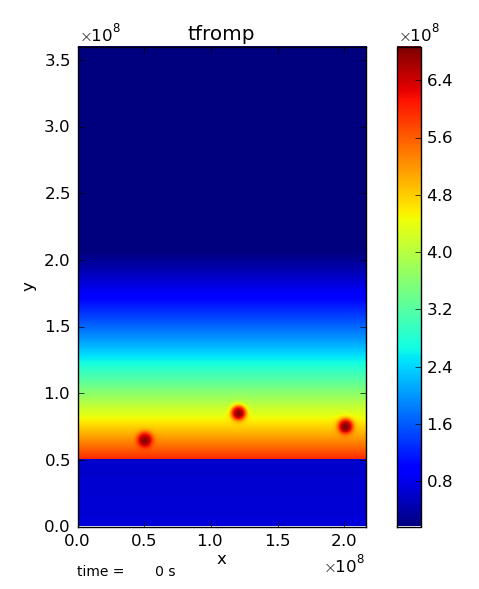
\includegraphics[height=0.4\textheight]{\visfigpath/plt00000_tfromp}
\caption[Basic plot of {\tt reacting\_bubble} done with {\tt plotsinglevar.py}]
{\label{fig:python} Plot of {\tt reacting\_bubble} done with the python
  script {\tt plotsinglevar.py}.}
\end{figure}

If you list 2 different variables after the plotfile name, then they
will be plotted side-by-side in a single figure.  For example, 
\begin{verbatim}
plotsinglevar.py plt00000/ tfromp enucdot
\end{verbatim}
produces the output shown in figure~\ref{fig:python_two}.

\begin{figure}[t]
\centering
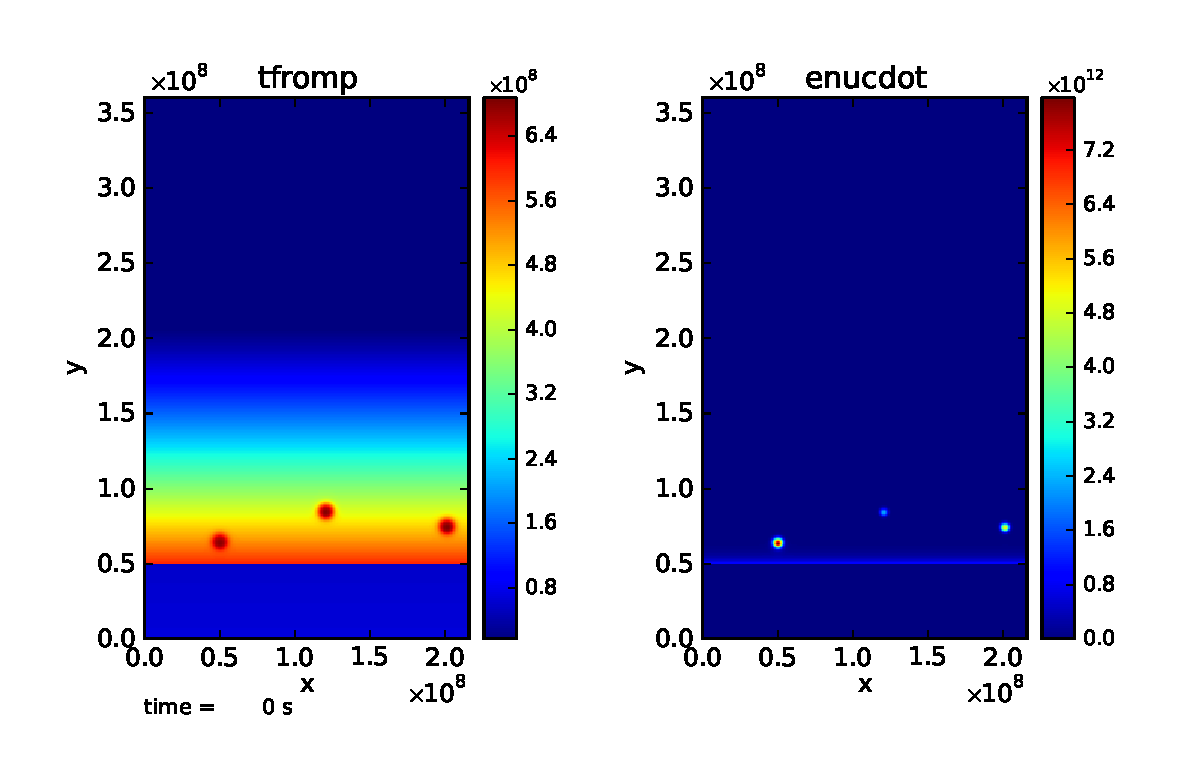
\includegraphics[height=0.4\textheight]{\visfigpath/plt00000_tfromp_enucdot}
\caption[Plot of two variables from {\tt reacting\_bubble} done with {\tt plotsinglevar.py}]
{\label{fig:python_two} Plot of {\tt reacting\_bubble} done with the
  python script {\tt plotsinglevar.py} showing 2 variables plotted
  from a single plotfile.}
\end{figure}


Additional options include `{\tt -m}' to specify the minimum data
value, `{\tt -M}' to specify the maximum data value, and `{\tt --eps}'
to make an EPS plot instead of PNG.  Running the script with no parameters
will give the full list available options.


Limited 3-d support is available.  When run as with a plotfile name
and variable, it will plot slices ($x$-$y$, $x$-$z$, and $y$-$z$) 
through the center of the domain.  The option `{\tt --origin}'
will put the slices through the origin.


\subsection{\tt contourcompare.py}

{\tt contourcompare.py} takes two or three plotfiles and a single variable as arguments
and plots contours of the datasets on the same set of axes.  This is 
form comparisons of different runs.  Running the script with no parameters
will give the full list available options.

For example:
\begin{verbatim}
contourcompare.py tfromp plt00000 other_plt00000
\end{verbatim}
will make a contour plot of the variable {\tt tfromp} from the data in
{\tt plt00000} and {\tt other\_plt00000} shown on the same axes.  


\subsection{\tt runtimevis.py}

The {\tt runtimevis.py} script is designed to be run from a submission
script to produce plots from plotfiles as they are produced.  This is
accomplished by hooking it into the {\tt process} scripts described in
Chapter~\ref{ch:managingjobs}.

The script itself reads in an inputs file, {\tt vis.in}, that
describes the variables to plot.  From 1 to 6 variables can be
plotting from a plotfile.  The script does its best to organize them
in columns and rows to maximize the plot area.  The image is always
output at 1280$\times$720 pixels, corresponding to 720p HD resolution.
For each variable, a block of the form:
\begin{verbatim}
[varname]
min = 1
max = 2
log = 1
\end{verbatim}
is supplied.  If {\tt min} or {\tt max} are omitted, then the data
limits are computed automatically.  If {\tt log} is omitted, then no
log is taken of the data before plotting.  The script is then run as:
\begin{verbatim}
runtimevis.py plt00000
\end{verbatim}



%-----------------------------------------------------------------------------
% yt
%-----------------------------------------------------------------------------
\section{\label{sec:vis:yt} Visualizing with \yt}

\yt is a Python package for analyzing and visualizing simulation data.
Originally \yt was written for the {\tt Enzo} code, with focus on
cosmological simulation data.  It has since been refactored to remove
the specific {\tt Enzo}isms, and now can work on various data formats,
such as the BoxLib data from \maestro\ and \castro, HDF5 data
from {\tt FLASH}, and data from the SPH code {\tt Gadget}.  For more
information, see the \yt homepage at \url{http://yt-project.org/} and
\cite{yt}.

\noindent {\bf Note: for \maestro\ data, you need to use \yt 3.0 or later.}

Some sample scripts that use \yt\ with \maestro\ data are contained in 
{\tt MAESTRO/Util/yt/}.

\subsection{Installing \yt}
The easiest way to obtain \yt is through the use of an installation script:
\begin{lstlisting}[language=bash,mathescape=false]
> wget http://hg.yt-project.org/yt/raw/yt-3.0/doc/install_script.sh
> bash install_script.sh
\end{lstlisting}
By default, this \yt install script will download and install, in its
own isolated environment, all the secondary utilities needed to get
\yt up and running.  Note that this currently includes installing {\it
  hdf5, zlib, bzip2, libpng, freetype, python, numpy, matplotlib,
  mercurial, ipython, h5py, Cython, Forthon} as well as a \yt {\it
  mercurial} bundle of changes.  You can turn off the automatic
installation of any of these particular packages by setting the
appropriate {\tt INST\_}* variable to zero in the install script; you
may have to then change some of *{\tt \_DIR} variables to point to
your own particular installation of that package.  It is usually best
to just let \yt install its own stuff, which ensures things are
working properly.

After the install script has finished, and assuming you let \yt
install its own packages, you'll need to {\it prepend} some
environment variables with \yt locations so that your system finds
those first and stops looking.  \yt provides a simple script to
do this, which will be announced upon successful completion.

%% \begin{lstlisting}[language=bash,mathescape=false]
%% # yt stuff
%% export YT_DEST=~/install/yt/current/yt-x86_64
%% export PATH=${YT_DEST}/bin/:$PATH
%% export PYTHONPATH=${YT_DEST}/lib/python2.6/site-packages/:$PYTHONPATH
%% export LD_LIBRARY_PATH=${YT_DEST}/lib/:$LD_LIBRARY_PATH
%% \end{lstlisting}
%% where I have {\tt ~/install/yt/current} as a soft link to my \yt
%% installation directory.

\subsection{Working with \yt}
The \yt installation provides both an interactive, {\it iPython}-like,
interface or the ability to import \yt modules for use in a batch
script.  The interactive interface should be in your {\tt \$PATH} if
you've followed the instructions in the previous section; to start it,
simply type {\tt iyt} in a terminal.
\begin{lstlisting}[language=Python]
> iyt

Welcome to yt!


In [1]: 
\end{lstlisting}
Codes like {\tt Enzo} use what are called {\it parameter files} to
describe the general information---number of levels, domain
dimensions, time, etc.---of a a dataset.  \yt likes to grab this
information before working on any specific data; this is accomplished
via the convenience method \textcolor{blue}{\tt load}:
\begin{lstlisting}[language=Python]
In [1]: pf = load("plt00166")
\end{lstlisting}
Note that some older versions of \yt needed an {\tt inputs} file 
in the same directory as the plotfile, but as of \yt 3.0, all the
necessary metadata is obtained from the {\tt job\_info} file inside
the plotfile directory.
The {\tt load} method returns an instance of the {\tt StaticOutput} class.  One
of the easiest ways of handling plots is via a {\tt PlotCollection}
object
\begin{lstlisting}[language=Python]
In [2]: center = (pf.domain_right_edge + pf.domain_left_edge) / 2.0
In [3]: pc = PlotCollection(pf,center)
\end{lstlisting}
By default, the {\tt PlotCollection} constructor places the center of
the plot to be at the location of peak density.  Here we have
calculated the center of the domain by accessing the lower and upper
domain boundaries via the {\tt numpy} arrays {\tt
  pf.domain\_left\_edge} and {\tt pf.domain\_right\_edge},
respectively.  Note that up until this point, \yt has not actually
loaded the AMR dataset.

Now we would like to take some slices of tfromp in the dataset and
generate some 2-d plots.  To do this, we will use the {\tt
  PlotCollection}'s \textcolor{blue}{\tt add\_slice} method:
\begin{lstlisting}[language=Python]
In [4]: pc.add_slice("tfromp",0)
In [5]: pc.add_slice("tfromp",1)
In [6]: pc.add_slice("tfromp",2)
\end{lstlisting}
The first call to \textcolor{blue}{\tt add\_slice} builds an {\tt
  AMRHierarchy} object associated with {\tt pf}.  The {\tt
  AMRHierarchy} object contains information about the actual dataset,
such as its layout in the simulation domain or on disk.  Building the
hierarchy is expensive, but once it is built the data it contains can
be accessed via attributes and dictionary lookup.  In other words, the
subsequent \textcolor{blue}{\tt add\_slice} operations are relatively
cheap.  The first parameter to the \textcolor{blue}{\tt add\_slice}
method is obviously the variable we want; the second (optional)
parameter specifies an coordinate axis orthogonal to the slice being
made---0 for x, 1 for y, 2 for z.  Now we want to save the plots from
the {\tt PlotCollection}; this is done with the \textcolor{blue}{\tt
  save} method, which takes an optional basename for the generated files:
\begin{lstlisting}[language=Python]
In [7]: pc.save("my_cool_images")
\end{lstlisting}
This generates the following image files:
\begin{lstlisting}[language=Python]
Out[7]: 
['my_cool_images_Slice_x_tfromp.png',
 'my_cool_images_Slice_y_tfromp.png',
 'my_cool_images_Slice_z_tfromp.png']
\end{lstlisting}
Figure \ref{fig:yt_slice} shows an example of one of the slice images.
Note that this was a quick and dirty generation of the image---there
is a lot of space around the figure, which can be removed with various
options to the \yt methods.  Also, the user can specify derived
variables, log-scaling, annotations, etc. For more information see the
documentation at \url{http://yt-project.org/docs/dev/}\, .

\begin{figure}[!h]\label{fig:yt_slice}
\centering
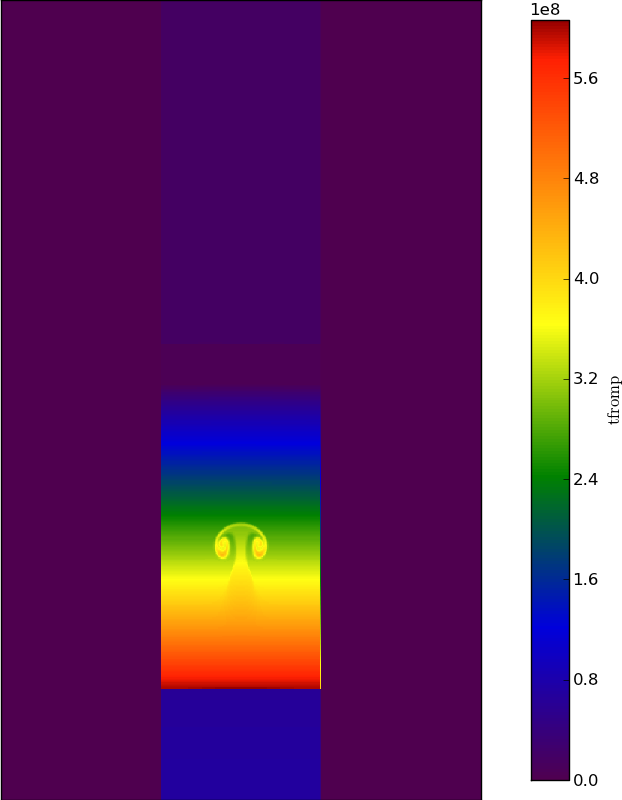
\includegraphics[height=0.4\textheight]{\visfigpath/my_cool_images_Slice_x_tfromp_trim}
\caption{Example slice through 3-d dataset with \yt.}
\end{figure}

When writing a script to use in batch mode, one has to manually import
the import modules needed to work with \yt.  As such, all scripts must
import from the {\tt yt.mods} module, which is essentially a
convenience module that sets up the appropriate \yt namespace.  
%% As an aside, if you want to import a module as another variable in
%% the local namespace---e.g. {\tt import this.module as
%% local\_variable}---then this should be done via the various API's
%% for that particular piece of code.  For example,
For completeness, below is a script containing our example above.
\begin{lstlisting}[language=Python]
# load our namespace
from yt.mods import *

# the plotfile I'm interested in
fn = "plt00166"

# load it into a StaticOutput object
pf = load(fn)

# find the center of the domain
center = (pf.domain_right_edge + pf.domain_left_edge) / 2.0

# associate a PlotCollection with the pf
pc = PlotCollection(pf,center)

# add some slices of tfromp
pc.add_slice("tfromp",0)
pc.add_slice("tfromp",1)
pc.add_slice("tfromp",2)

# save our plots to a files with basename
# "my_cool_images"
pc.save("my_cool_images")
\end{lstlisting}

\subsection{2-d datasets}

To visualize 2-d data, you can use the {\tt SlicePlot} function,
picking the normal direction to be {\tt "z"}:
\begin{lstlisting}
from yt.mods import *
 pf = load("plt00085")
s = SlicePlot(pf, "z", "tfromp")
s.save("tfromp.eps")
\end{lstlisting}
This generates the figure shown in Figure~\ref{fig:yt2d}.

\begin{figure}[!h]
\centering
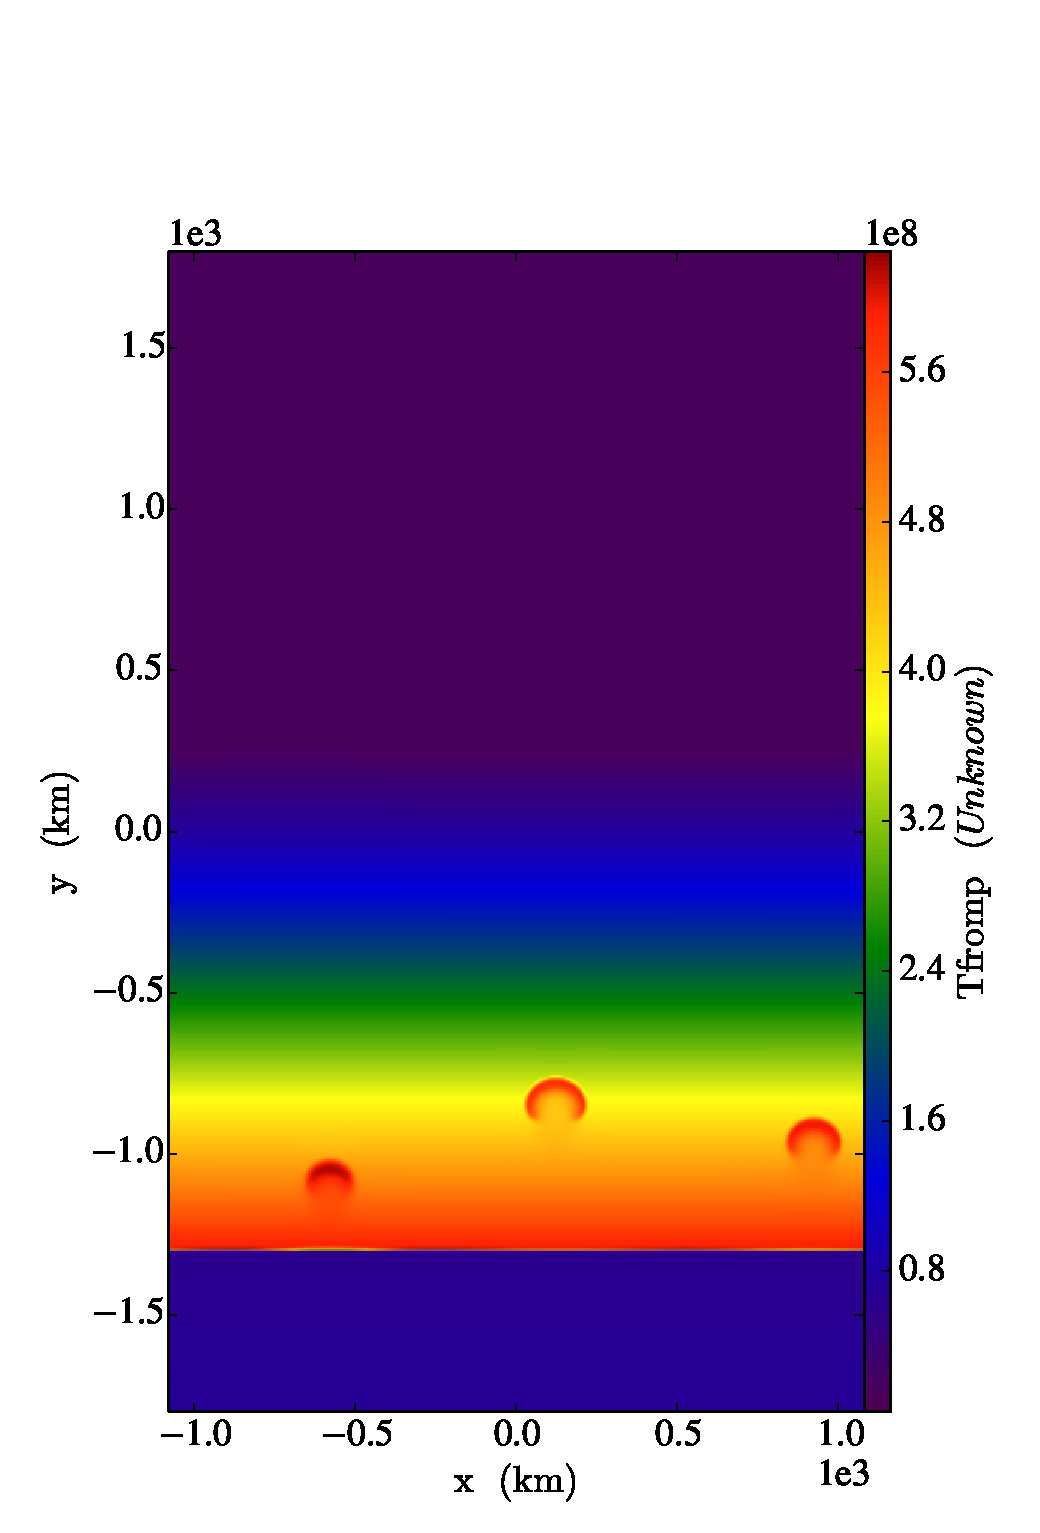
\includegraphics[height=0.4\textheight]{\visfigpath/tfromp}
\caption{\label{fig:yt2d} Example slice through 3-d dataset with \yt.}
\end{figure}

\subsection{Volume Rendering}

